%VETB Report
\documentclass{report}
\author{Tym Pakulski - University of Bath}
\title{Internal Volume Measurement Device}
\date{September 2013 - August 2014}

\usepackage{graphicx}
\usepackage{amsmath}
\setlength{\parindent}{0pt}
\begin{document}
\graphicspath{{./images/}}
\maketitle
\tableofcontents
\section{Introduction}
Leak testing of the various CMS cooling systems is a regular exercise that currently relies on a 'rule of thumb' approach to test specifications. True allowable leak rates are defined in terms of a percent of total internal volume per unit time, but exact numbers for the internal volumes of the various subsystems are difficult to establish. A device that can measure the internal volume of existing systems would be useful to quantify allowable leak rates and streamline the leak testing process.
This report documents the proof-of-concept phase of a rig that will be used to measure internal volumes by injecting them with gas and measuring the rate of pressure change. 
\subsubsection{Useful Contacts}
\begin{itemize}
	\item{Norbert Frank: +41764873618, Norbert.Frank@cern.ch }
	\item{Patrick Carrier (for instrumentation): +41764870415, Patrick.Carrie@cern.ch}
	\item{Roberto Guida (for theory): +41764872146, Roberto.Guida@cern.ch}
	\item{Tym Pakulski: tsp26@bath.ac.uk}
\end{itemize}
\subsection{Theory}\label{theory}
The volume measurement concept comes from the ideal gas law \eqref{ideal}, and the equation for molar volume \eqref{molarVolume}. It assumes constant temperature and volume. All units are S.I.

\begin{eqnarray}
PV = nRT \label{ideal}\\
V_{mol} = \frac{RT}{P} \label{molarVolume}\\
n = \frac{PV}{RT} \nonumber \\
\frac{dn}{dt} =  \frac {V}{RT} \frac {dP}{dt} \nonumber \\
\frac{dV_{in}}{dt} =  \frac{RT}{P} \frac {V}{RT} \frac {dP}{dt} \nonumber \\
V = \dot{V_{in}} dt \frac{P_1}{P_2 - P_1} \label{tym}
\end{eqnarray}
An alternative derivation supplied by Roberto Guida assumes standard conditions to calculate the molar volume. While slightly more complex, this formulation has the advantage of taking flow controller readings directly as input, as it corrects for ambient temperature different from the flow controller calibration. See \ref{sec:operatingPrinciples}.
\begin{eqnarray}
PV = nRT \nonumber\\
V_{mol} = 22.4 \text{ [L]}\\
n = \frac{PV}{RT} \nonumber \\
\frac{dn}{dt} =  \frac {V}{RT} \frac {dP}{dt} \nonumber \\
\frac{dV_{in}}{dt} =  \frac{22.4}{R} \frac {V}{T} \frac {dP}{dt} \nonumber \\
\dot{V}_{in}\text{ [l]} = 2.69\frac{V}{T} \frac{P_2 - P_1}{dt} \nonumber \\
V = \frac{\dot{v}_{in}}{2.69} \frac{T}{P_2 - P_1}\nonumber \\
V\text{ [cm$^3$]} = \frac{\dot{v}_{in}\text{ [l/hour]}}{3600}\frac{dt\text{ [s]}}{P_2-P_1 \text{ [bar]}}\frac{T\text{ [$\,^{\circ}\mathrm{C}$]}+273}{269}1000 \label{roberto}
\end{eqnarray}
The concept can be implemented by moving gas from a high-pressure volume to the test volume at a known constant rate and measuring the change in pressure over time. The minimum apparatus to achieve this involves a pressurised gas bottle connected to a flow controller and a downstream pressure sensor, as shown in Figure \ref{schematic}.
\begin{figure}[h]
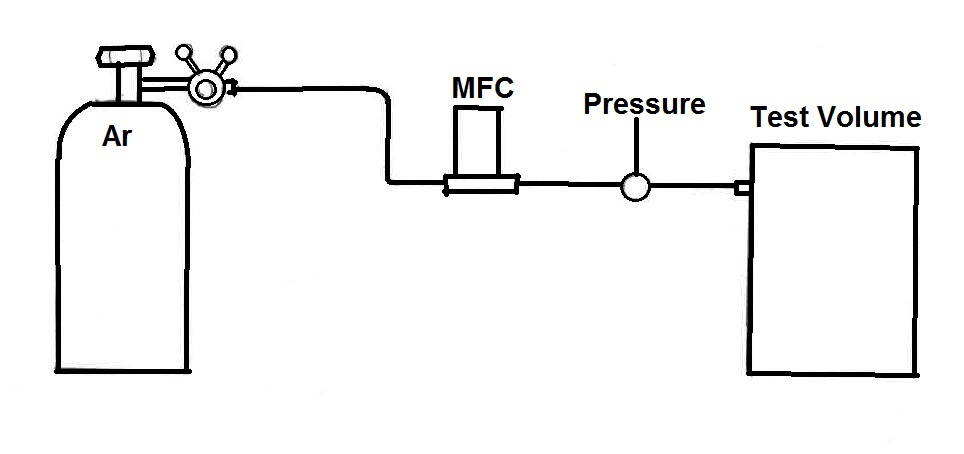
\includegraphics[width=\textwidth]{schematic}
\caption{Schematic of the volume estimation concept}
\label{schematic}
\end{figure}
\\
\subsection{Specifications}
The final product should be:

\begin{itemize}
	\item{Compact and transportable}
	\item{Simply designed and accessible for untrained users}
	\item{Sufficiently accurate to meet the leak test specification accuracy}
	\item{Functional without a laptop or expensive data logging equipment}
	\item{Self-sufficient in DAQ and practical for automated data analysis.}
\end{itemize}

\subsection{Accuracy Specification}
The accuracy of the device is constrained by the allowable errors in the device's uses. An error in the calculated volume will affect the accuracy of both the \textit{allowable} leak rate and the \textit{measured leak rate}.\cite{leakPaola}.
%ACCURACY SPEC

\subsubsection{Error Prorogation}
Errors in estimated volume arise from two sources:
\begin{itemize}
\item{Pressure: a combination of read error and storage error of the 4-20 mA signals.}
\item{Flow Rate: Deviations from the set point. The theoretical worst case scenario can be expressed as a constant systematic error equal to the maximum random error.}
\item{Time is considered perfectly accurate.}
\end{itemize}
From equation \ref{tym}, let:
\begin{itemize}
\item{$\epsilon$ = the absolute error in calculated volume}
\item{$\delta$ = the absolute error in pressure}
\item{$\gamma$ = the absolute error in flow rate}
\item{$\delta << P$}
\item{$\gamma<< \dot{V}_{in}$}
\end{itemize}
Then:
\begin{eqnarray}
V \pm \epsilon= (\dot{V_{in}}\pm \gamma) dt \frac{P_1\pm \delta _1}{P_2 \pm \delta _2 - P_1 \pm\delta _1} \nonumber \\
V \pm \epsilon = \frac{\dot{V}_{in} dt P_1}{dP \pm \delta _1 \pm \delta _2} \pm \frac{\gamma dt P_1}{dP \pm \delta _1 \pm \delta _2}\pm\frac{\dot{V}_{in}dt \delta _1}{dP \pm \delta _1 \pm \nonumber \delta _2}\pm \frac{\gamma dt \delta _1}{dP \pm \delta _1 \pm \delta _2} \nonumber \\\\
\text{From assumptions: } \nonumber\\
V \pm \epsilon = \frac{\dot{v}_{in} dt P_1}{dP} \pm \frac{\gamma dt P_1}{dP}\pm\frac{\dot{V}_{in}dt \delta _1}{dP} \nonumber\\\\
\text{Equivalent to: } \nonumber \\ \\
V =  \frac{\dot{V}_{in} dt P_1}{dP} \nonumber \\ 
\epsilon = \pm \frac{\gamma dt P_1}{dP}\pm\frac{\dot{V}_{in}dt \delta _1}{dP} \nonumber\\
\frac{\epsilon}{V} = \frac{\pm \frac{\gamma dt P_1}{dP}\pm\frac{\dot{V}_{in}dt \delta _1}{dP}}{\frac{\dot{V}_{in} dt P_1}{dP}}\nonumber \\
\frac{\epsilon}{V} = \pm \frac{\gamma}{\dot{V}_{in}} \pm \frac{\delta _1}{P_1}\\
\end{eqnarray}

	
\section{State of the Project}
So far, the volume estimation concept has been tested using a pressure transmitter and DAQ of Norbert Frank's pressure decay measurement rig in building 27, shown in Figure \ref{b27}. Two different flow controllers have been used to measure the volume of a dive bottle. 
\begin{figure}[h]
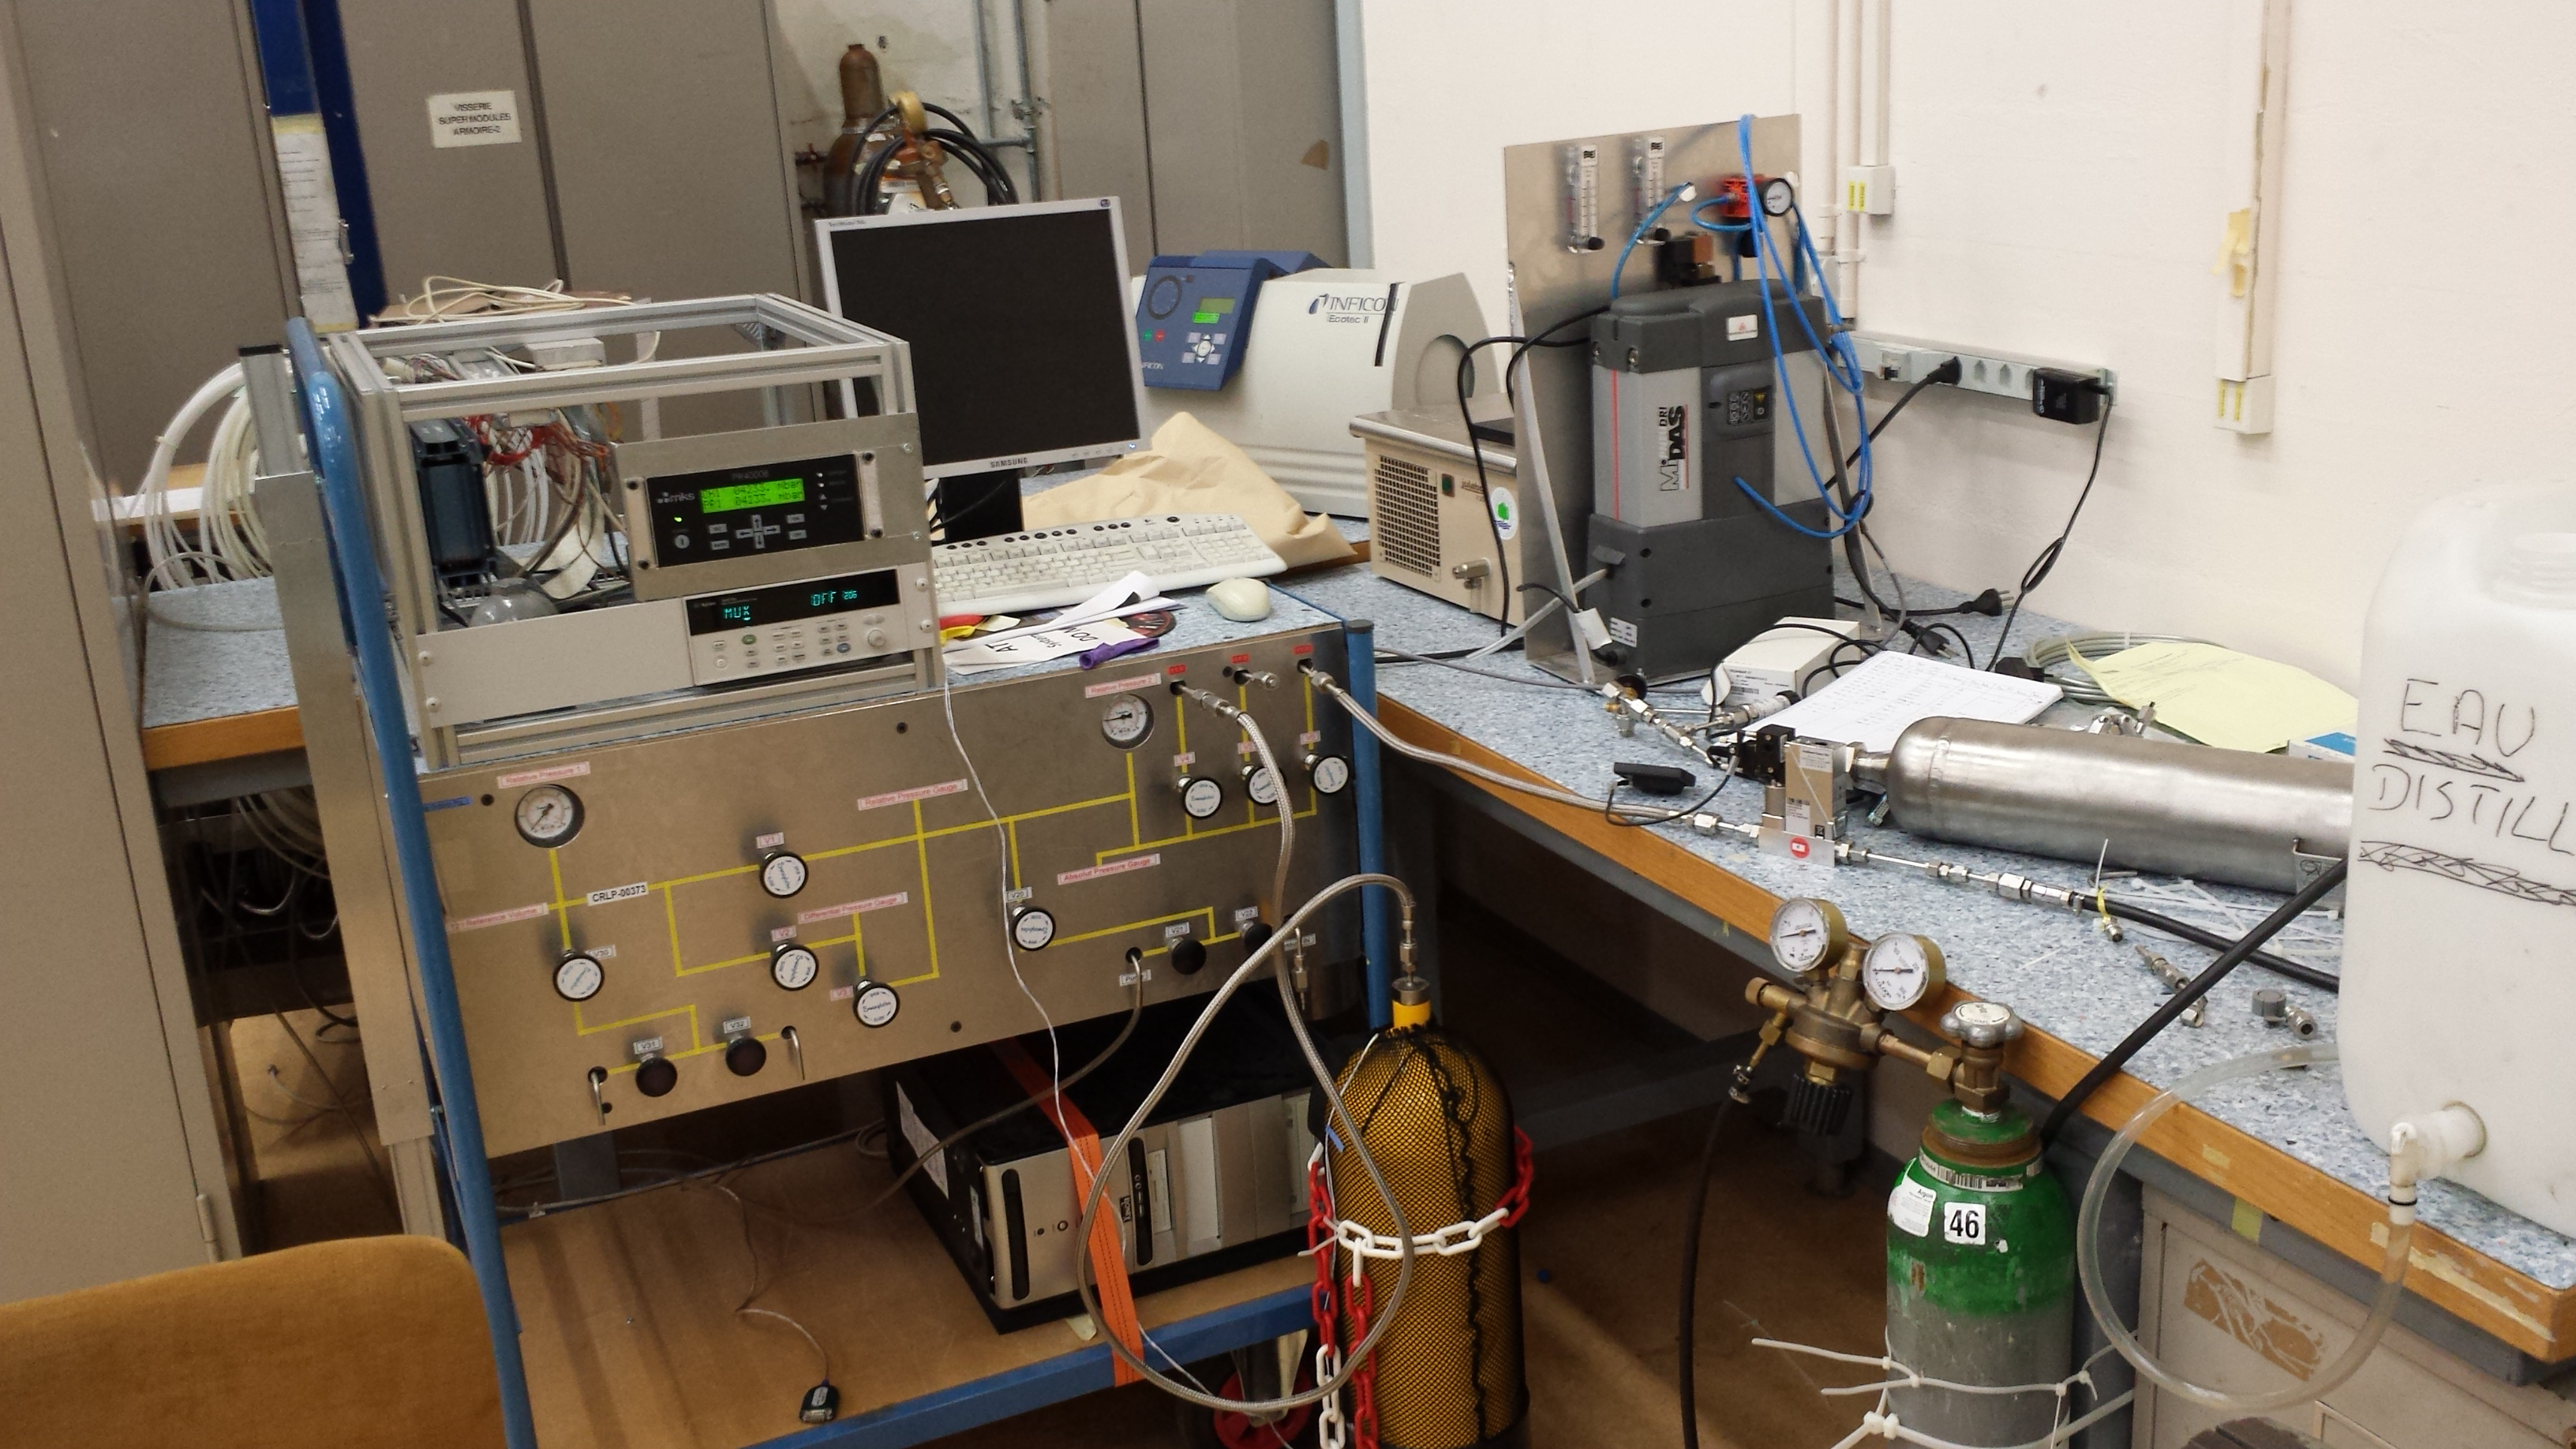
\includegraphics[width = \textwidth]{wide}
\caption{The test rig in building 27.}
\label{b27}
\end{figure}
\subsection{Using the Building 27 Rig}
DAQ is handled by a \textit{labVIEW} module on the local PC. The \textit{.vi}, accessible from \textit{Desktop}, is called \textit{MAIN\textunderscore ScanChannels.vi}. Tests can be run from the \textit{Stand1} tab on the front panel. The data for each test is saved to a .txt file in a folder at \textit{C:/Project/PressureTest/Data/}. The useful channels are the time and the first pressure signal: \textit{absSysPressure}. The PC also has installed Bronkhorst's Flow DDE and Flow Plot software, which can be used to change the flow controller set point and log its 3 channels through RS232.The current flow controller is connected to a local display for adjusting the set point. The password for the display is \textit{abc}. \\
The rig is connected to the 15 L (true volume) dive bottle with 1/4" VCR fittings. The bottle's volume was confirmed by filling it with water and measuring its change in weight. \\
The rig's gas inlet, purge line and fluid connection are controlled by valves shown in Figure \ref{valves}.

\begin{figure}[h] 
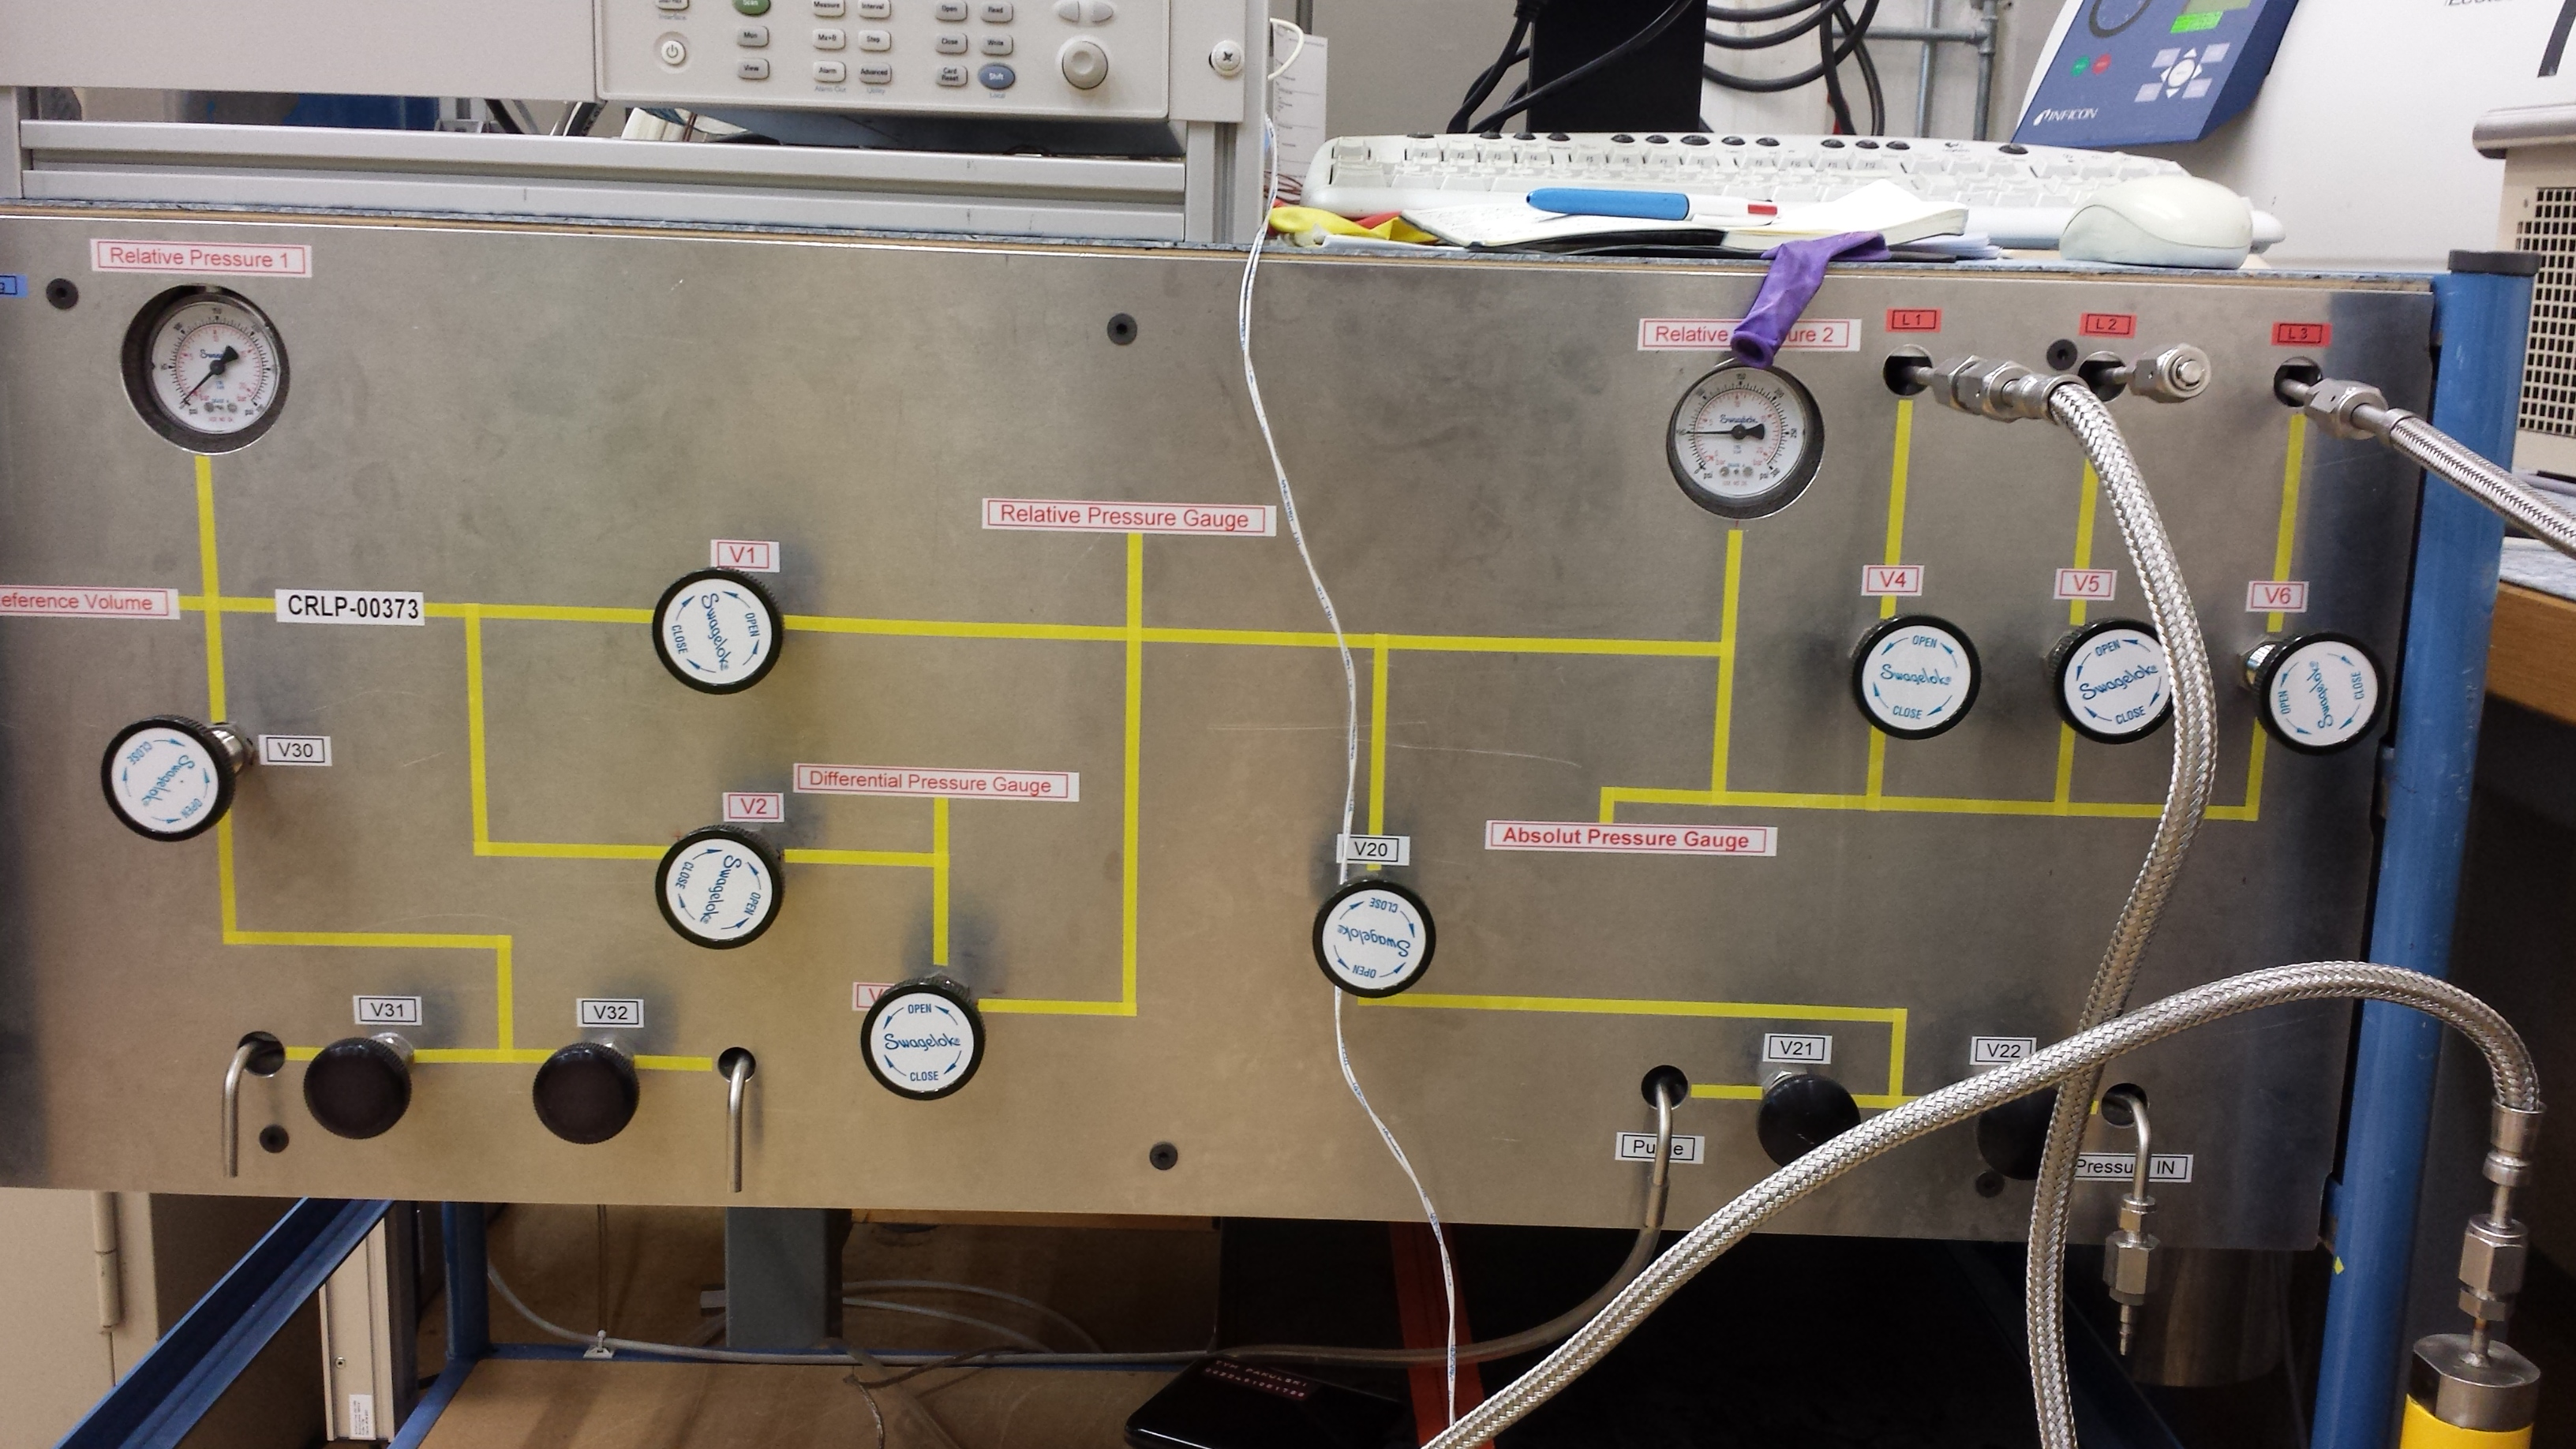
\includegraphics[width=\textwidth]{valves}
\caption{V6: fluid inlet, V4: Test volume, V20 and V21: Purge, V1 and V3: keep closed}
\label{valves}
\end{figure}

Valve 4 connects to an unused part of the rig and is kept close to minimise pipe volume.\\
\subsubsection{Running a Test}
To run a test, open the \textit{Stand1} tab of \textit{MAIN\textunderscore ScanChannels.vi}, as shown in Figure \ref{labVIEW}. Type in a name for the test and a start pressure. And click run. 
\begin{figure}[h]
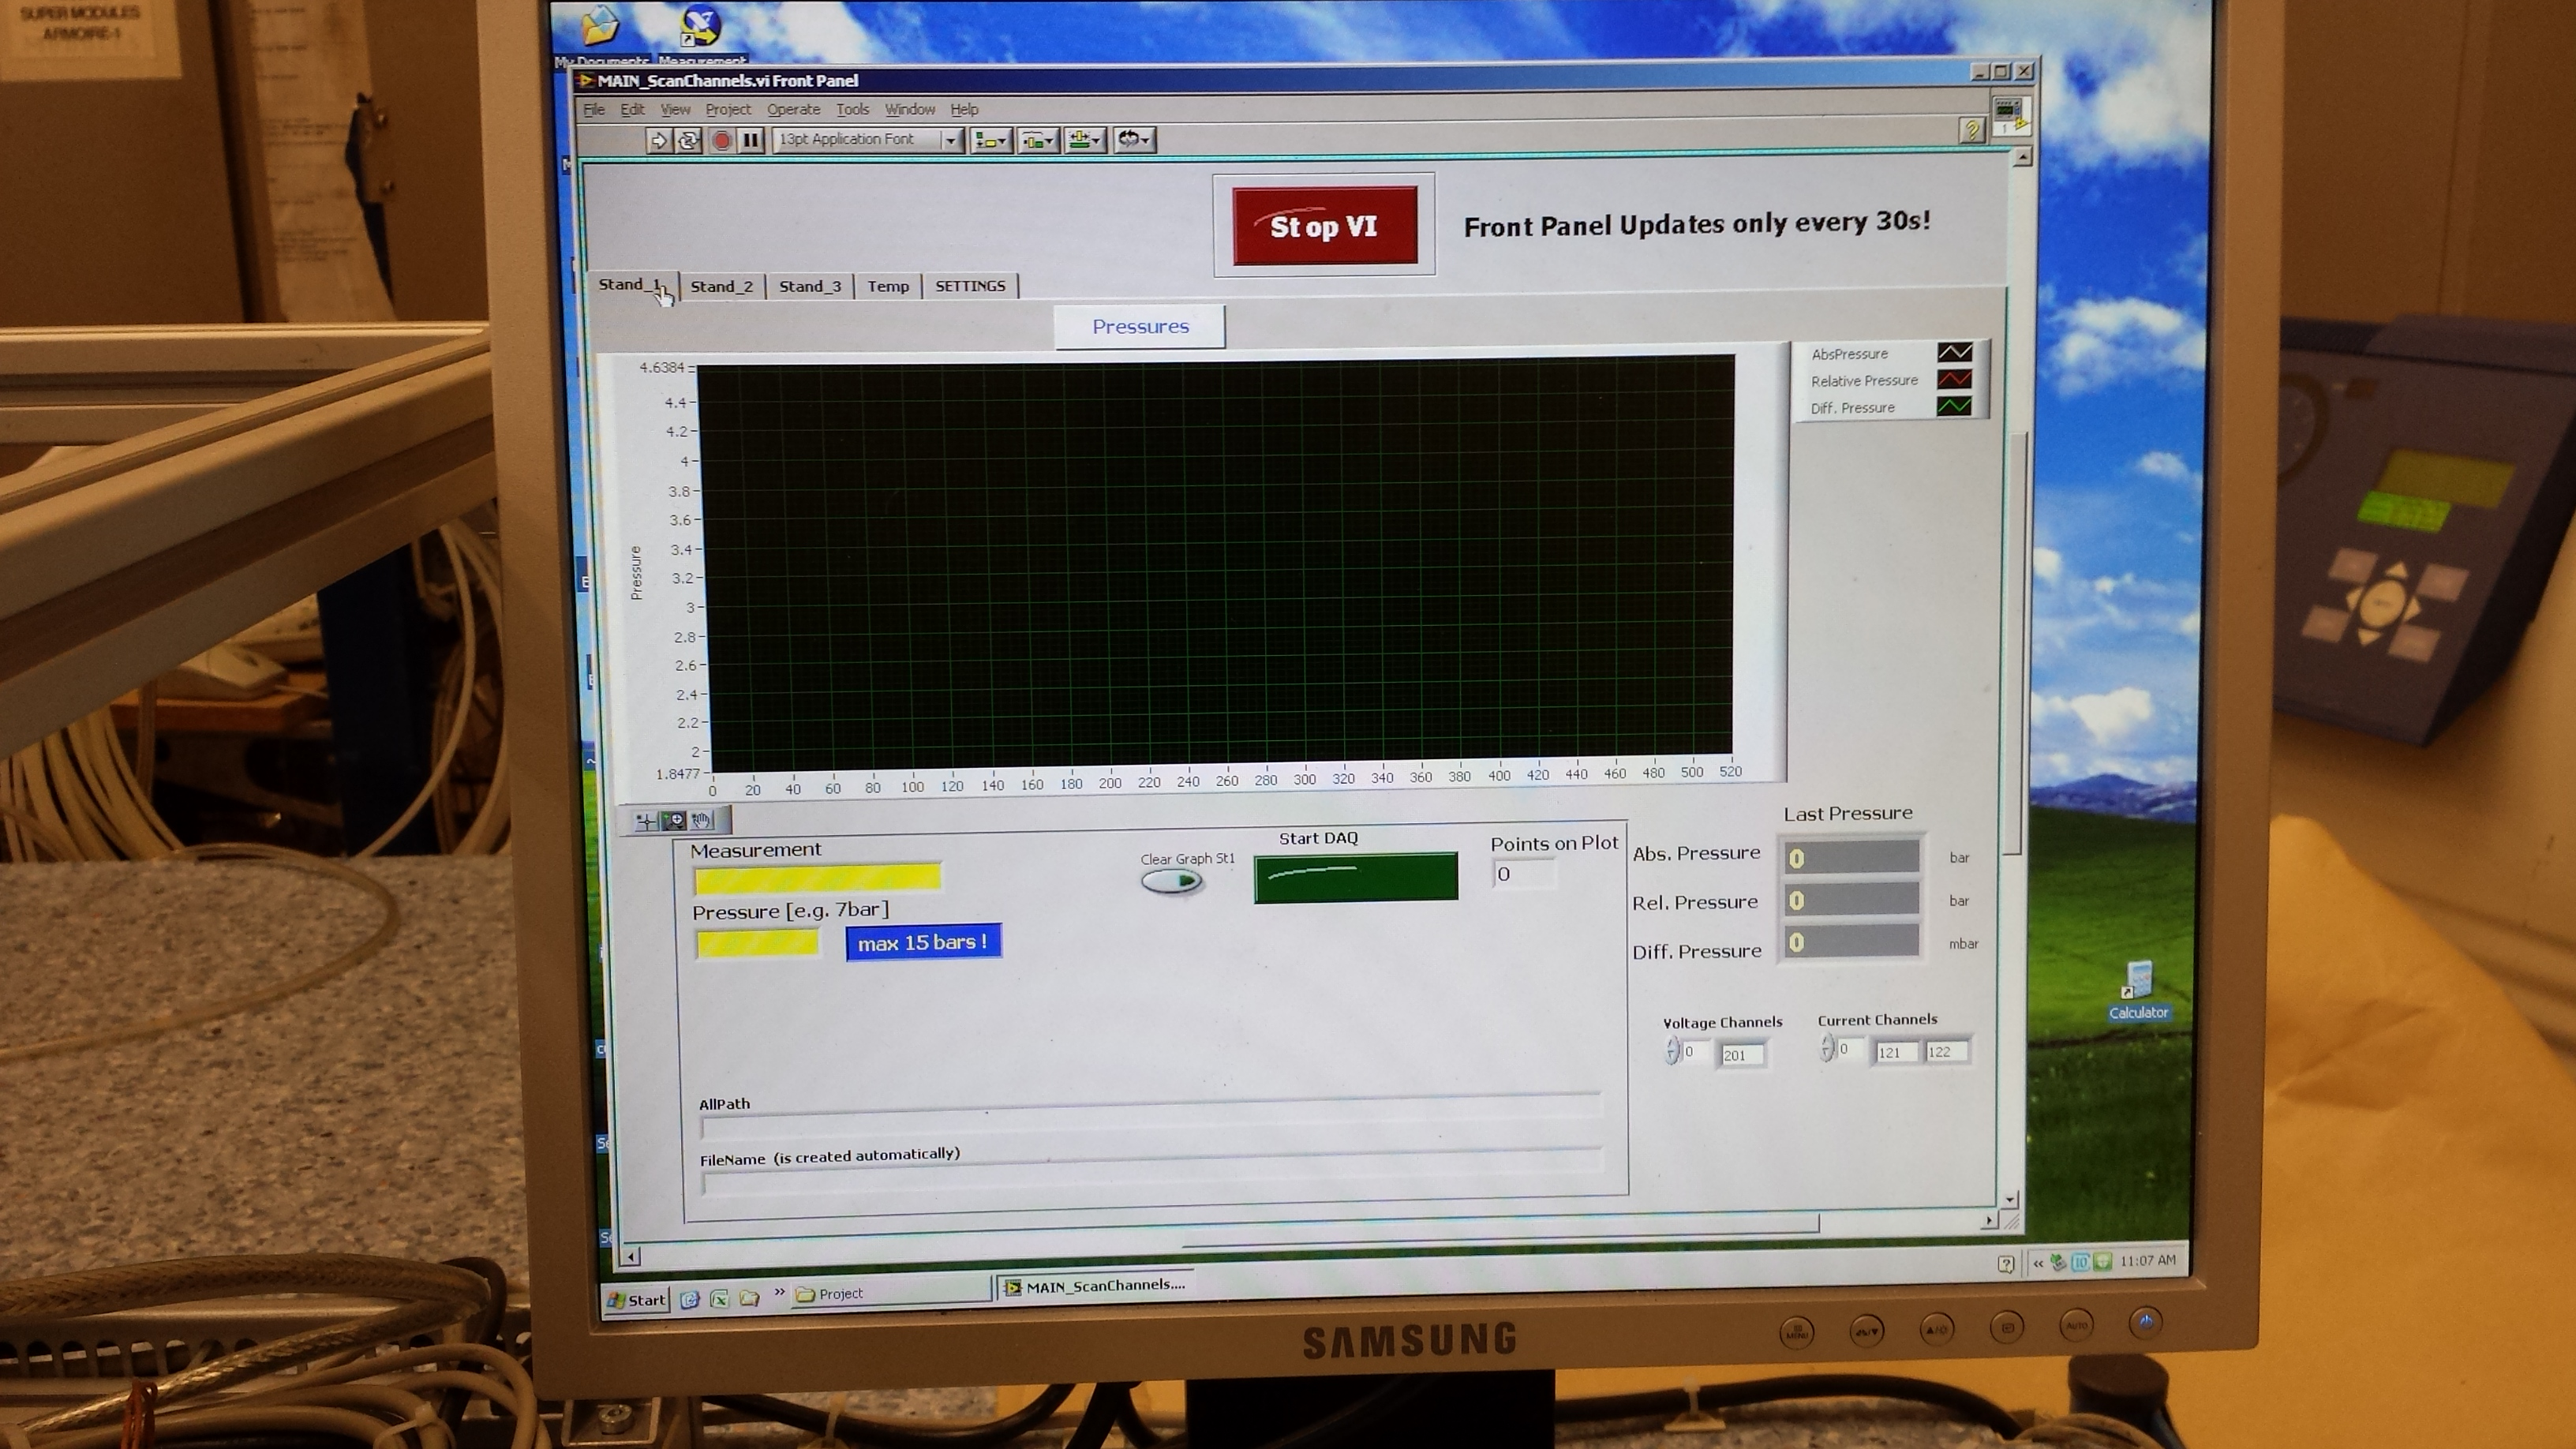
\includegraphics[width =\textwidth]{labVIEW}
\caption{The \textit{MAIN\textunderscore ScanChannels.vi} front panel. Red labels have been added for clarity.}
\label{labVIEW}
\end{figure}
Purge the system until it reaches atmospheric pressure and close the purge valve. Open the valve on the gas bottle, and adjust the pressure reducer to match the calibration pressure of the flow controller. Then, adjust the set point of the flow controller. Ensure that the valve between the pressure reducer and the flow controller is open, and the purge and differential valves on the rig are closed. Click the green button \textit{Start DAQ}.
\subsubsection{Historical Data}
All historical data is available on the PC linked to the test rig at \textit{C:/Project/PressureTest/Data/}. However, the various tests are poorly organised. You can find structured data at \textit{G:/Departments/PH/Groups/DT/PO/Cooling activities/students/tpakulsk/VETB}. The data is organised in to 4 series: \textit{VETB1, VETB2, VETB3} and \textit{VETB4}. In general, data from \textit{VETB1} is of little use, as many of the tests were voided by incorrect inlet pressure and other problems with execution. The remaining three folders following the a naming convention:\\
\subsubsection{Naming Convention}
The name of each .txt file from labVIEW or Flowplot denotes the test series, flow rate, test repetition and the signal being measured. The first character of the name represents the test series: A for VETB2, B for VETB3 and C for VETB4. The following 4-character string is the flow rate set point in $ml_nmin^{-1}$. The next digit represents the repetition of the test, and the final character is F for flow data from the controller serial bus or P for pressure data. An example is shown in \ref{namingConvention}.

\begin{figure}[h]

\includegraphics[width = 5cm]{namingConvention}
\caption{An example file name for VETB2, 55 $ml_nmin^{-1}$, second test, flow data}
\label{namingConvention}
\end{figure}



\section{Instrumentation and DAQ}
\subsection{Bronkhorst Flow Controllers}
The first iterations of the rig have used Bronkhorst \textit{EL FLOW} flow controllers. These were borrowed from Patrick Carrier of the Gas Group in building 155. 

\subsubsection{Flow controllers used}
\begin{tabular}{ p{2.4cm} | l l }
Controller: & EL FLOW 1 & EL FLOW 2\\
Used for: & VETB 1-3 & VETB 4 \\
Maximum Flow: [$lmin^{-1}$]& 0.1 & 1 \\
Calibration P: [bar g]& 6 & 3 \\
Calibration T: [$\,^{\circ}\mathrm{C}$]& 20 & 20\\
Calibration fluid: & Ar & Ar\\
Leak tight: & Unlikely & yes\\
\end{tabular}
 
\subsubsection{Operating Principles} \label{sec:operatingPrinciples}
The controllers operate on the thermal mass flow principle, and measure the mass of fluid passing through their regulation valve as a function of the power needed to heat a temperature probe a set distance away in the flow. \cite{bronkhorst} The instruments take a $L_n$ per minute set point via RS232 bus, which they convert for their grams per second control logic using equation \eqref{molarVolume}. In other words, the instruments are calibrated for a specific fluid, inlet pressure and fluid temperature. \textbf{It is essential that these parameters are respected.}\\
\\
In practice, this means using the correct fluid and adjusting the downstream pressure of the reducer to match the value specified in the controller firmware and typically marked on the side of the device. \\Ambient temperature is more difficult to adjust. Instead, it is good practice to check the calibration temperature, which is typically 293 K, and multiply the volumetric flow rate by a 'temperature gain' using equation \eqref{temperatureGain}.
\begin{equation} \label{temperatureGain}
\dot{V}_{true} = \dot{V}_{set point}\frac{T_{true}[K]}{T_{calibrated}[K]}
\end{equation}
\\
Alternatively, the temperature gain can be applied to the calculated volume itself. If the derivation supplied by Roberto Guida is used, the temperature difference can be ignored. \\

\section{Problems with Flow Controllers}
Two major problems were encountered during early iterations of the project. 
The first version of the instrumentation seemed to exhibit random errors in calculated volume in the order of 10\%, well beyond those predicted by theory. Second, an unexpected correlation between injection flow set point and calculated volume was observed. 
Both problems were resolved by a change of flow controller. \\ \\
It appears the most likely explanation for the systematic error is a leak in the instrumentation section. In general, a faster flow rate means a larger integral of pressure with respect to time, as shown in Figure \ref{both}. The leak rate is in turn proportional to the difference of the squares of the system pressure and ambient pressure \cite{leakPaola}, so it can be concluded that the net leak flow over a fixed time interval will be higher for a faster flow. From equation \ref{tym} it is clear that the higher leak flow leads to an overestimation in of volume.  
\begin{figure}[h]
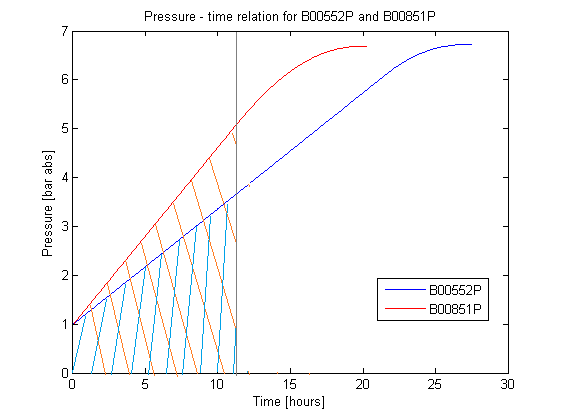
\includegraphics[width = \textwidth]{both}
\caption{Pressure-time relation for two different flow rates, note the greater integral of pressure for the higher flow rate.}
\label{both}
\end{figure}

Thus the higher the flow rate, the greater the error due to leaks. No leaks were found in several sniffer tests conducted with both $CO_2$ and helium. However, pressure decay in the instrumentation section consistent with a leak was observed. \\ \\
The random error in calculated volume was most likely due to temperature variations. At first, minor temperature variations seemed trivial. The temperature term is eliminated in the first formulation of the derivation used for data analysis, and can only be expressed as a pressure error using the ideal gas law. The resulting linear error implies that the typical 3 degree temperature fluctuations observed were insignificant. \\ \\ The problem with this conclusion is that the derivation itself rests on the assumption of constant temperature, and the 1 percent error is enough to invalidate the volume estimation concept completely. In other words, a small temperature variation voids the entire test. \\ \\
EL-FLOW 2, with 10 times the maximum flow of EL-FLOW 1,  eliminated the systematic error with leak tight connections, and allowed fast-flow tests too short for significant temperature fluctuations. While the old controller required 8-14 hour tests for the 15 L volume, the new one could achieve 4 bar of dP in 30 minutes. 
\subsection{Theoretical Understanding}
A lack of theoretical understanding of the exact operating principles of the flow controllers has hindered the accuracy of the rig. Specifically, the conversion from the mass flow rate measured by the controllers to the volumetric flow set point is poorly understood. The project would greatly benefit from a meeting with Patrick Carrier or Roberto Guida to understand exactly how the controllers convert from moles to volume, what parts of this conversion are taken care of by the analysis equations in \ref{theory} and where temperature gain must be applied.

\subsection{Full Scale Error}\label{fullScale}
According to the flow meter data sheets, the flow meters exhibit absolute random errors of 2\% \textit{full scale}.\cite{bronkhorst} This means that if their set point is their maximum flow, the relative random error is 2\%. But the relative error grows as the flow set point is reduced. For example, for EL-FLOW 2, at a set point of 0.1 $L_n/min$, the relative error is $\frac{0.02\times 1}{0.1} = 20\%$. This implies that instrumentation should whose upper range is appropriate for the volumes of interest should be selected to maximise accuracy.

\subsection{DAQ}
Estimating volume requires, at a minimum, two data points of time and pressure and the flow set point.
\begin{figure}[h]
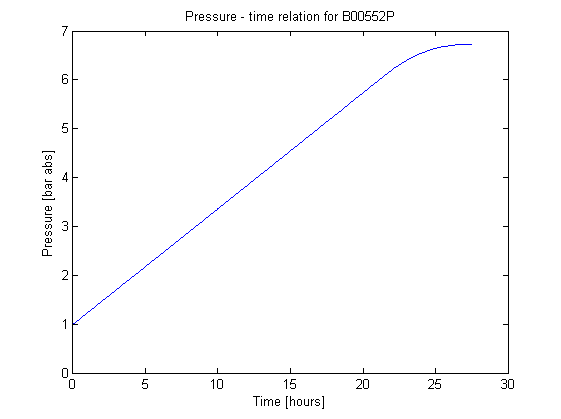
\includegraphics[width = \textwidth]{B00552P}
\caption{A typical pressure-time relation}
\label{typical}
\end{figure}
A temperature reading is useful to eliminate a minor systematic error if temperature is constant, or to detect a change in temperature that would void the test. More time and pressure data reduce random errors. \\
The current rig measure pressure through a 4-20 mA current loop connected to a \textit{LabVIEW} module. The software can log pressure and time in this way. Future iterations of the project will probably simplify the DAQ process by saving the current loop readings with timestamps to a USB storage device. This will allow the test to be run without a laptop. 
\section{Analysis tools}
Various analysis tools were used during different stages of research. Calculating volume from two time - pressure points is a simple process that can be done with a hand calculator. However, several tools were developed in Matlab and Python 3.3 to allow for repetitions of this calculation over different data sets or time intervals. The Python script \textit{cleanData.py} was used to iterate through different time intervals of a single data set, and calculate a volume for each one. The data could then be plotted in MS Excel. 
\subsection{Alternative Analysis: Slope Interpretation}
An alternative method for data analysis was explored theoretically but never implemented. The method relies on plotting the relation of pressure inside the test volume against time, and measuring the gradient to calculate the volume. It would eliminate the problem of random errors if two outlier points are selected for the calculation, as it takes into account all of the points in the test.\\ \\
From equation \ref{tym}:
\begin{eqnarray} \label{slopeDerivation}
V = \dot{V}_{in} dt \frac{P_1}{P_2 - P_1} \nonumber \\
\text{General case for \textit{P} as a function of \textit{t}:} \nonumber \\
V = \dot{V_{in}} t \frac{P_{start}}{P_{(t)} - P_{start}}\nonumber \\
P_{(t)} -P_{start} = \frac{\dot{V}_{in}t}{V} \nonumber \\
P_{(t)} = \frac{\dot{V}_{in}t}{V} +P_{start} \\
\text{gradient} = \frac{\dot{V}_{in}t}{V} \nonumber \\
V = \frac{\dot{V}_{in}}{\text{gradient}} \label{slopeInterpret}
\end{eqnarray}

After reading off the gradient of the linear region of a \textit{P} against \textit{t} relation, such as the one shown in Figure \ref{typical}, the test volume can be calculated using equation \ref{slopeInterpret}.

%WHERE TO FIND MATLAB ETC
%PYTHON SCRIPTS


\section{Recommendations}
The next iteration of the product should evaluate its accuracy for smaller test volumes of 2-3 litres. If the system's performance meets accuracy specifications, focus can shift to selecting permanent components with the correct parameters.

Future iterations should respect the following findings about the instrumentation
\begin{itemize}
	\item The inlet pressure on the flow meter must match the calibration pressure  in the firmware.
	\item The test volume temperature must be kept constant.
	\item Tests should be kept short to minimise temperature variation. 
	\item A temperature gain should be applied to the calculated volume if rig temperature differs from the calibrated temperature.
	\item A fast flow meter in the order of 1 l/min appears to offer a good balance of short test duration and flexibility for test volumes of interest.
	\item The flow controller should be selected so that the appropriate set point is close to the maximum flow. This will minimise relative errors due to the full-scale absolute error discussed in \ref{fullScale}.
	\item The rig must be leak tight.
	\item The project will require a deeper understanding of the theory, especially the conversion between moles per second and $l_ns^{-1}$ made by the mass flow controllers. To decide which equation will be implemented in the future and how temperature deviations will be handled.
\end{itemize}	
With instrumentation ordered, final design development should focus on the user experience, specifically the software. With 4-20 mA current readings saved to a USB drive, a simple program should be written to fetch and analyse the data.
Once a minimum viable product has been established, two further developments are worth investigating:
\subsubsection{Monitoring temperature} 
A temperature measurement is useful to be able to quantify the temperature gain that should be applied to the volume calculation to account for the difference in gas temperature and calibration temperature. Further, a running temperature measurement can be used to check whether significant temperature changes occur during the test, which would void the data.\\
The former could be achieved with something as simple as an analogue thermometer somewhere on the rig, assuming a constant temperature throughout the test. The latter would require dedicated hardware and DAQ to store the signals, which would likely be incompatible with the 4-20 mA pressure signals. With short tests, it can be argued that it is safe to assume constant temperature throughout the test.
\subsubsection{Pressure decay test capability}
The rig could also be used for pressure decay testing. By adding a valve upstream of the pressure sensor as shown in Figure \ref{schematicWithValve}, the pressurised test volume can be sealed, and the pressure transducer can be used to record pressure drop over time.\cite{leakPaola} 
\begin{figure}[h]
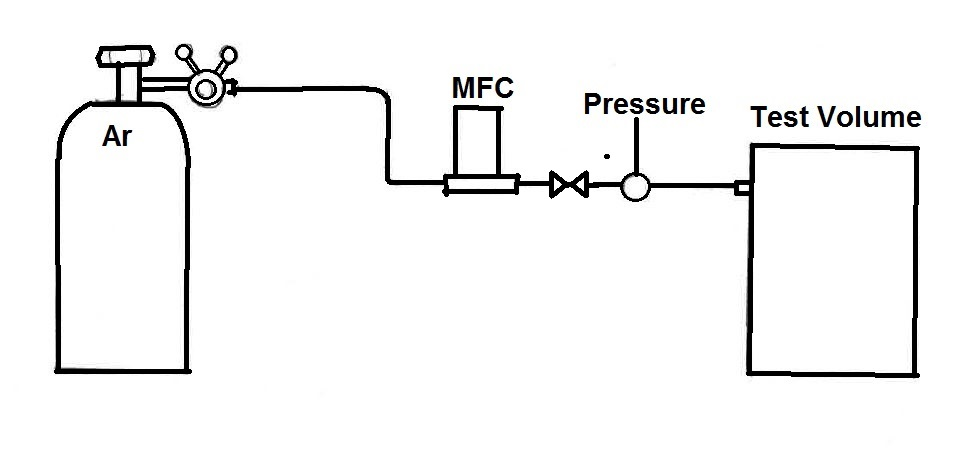
\includegraphics[width=\textwidth]{schematicWithValve}
\caption{The volume estimation instrumentation with an added valve for pressure decay testing.}
\label{schematicWithValve}
\end{figure}
This would could prove particularly convenient in the CMS, as it would allow both the volume estimation and the pressure decay test without purging the system or disconnecting the fittings. The device would first be connected to the pressure reducer and the test volume. Argon would be injected and pressure measured to calculate the volume. Then, the valve would be closed and pressure drop measured. With the pressure drop, the time, and the calculated volume, the leak rate can be calculated. 

\begin{thebibliography}{1}
\bibitem{leakPaola} Paola Tropea {\em Procedures for the Construction and Testing of the Cooling Plants Built by the TS/CV/DC Section} 2006: TS Department, CERN
\bibitem{bronkhorst} Bronkhorst High-Tech {\em EL-FLOW Digital Thermal Mass Flow Meters and Controllers for Gases} http://www.bronkhorst.com/files/downloads/brochures/folder-el-flow.pdf
\end{thebibliography}
\end{document}


